\documentclass[11pt]{article}
\usepackage[utf8]{inputenc}
\usepackage{fancyhdr}
\usepackage[english]{babel}
\usepackage{latexsym}
\usepackage{graphicx}
\usepackage{array}
\usepackage{amsmath}
\usepackage{amssymb}
\usepackage{mathtools}
\usepackage{algorithmicx}
\usepackage{algpseudocode}
\renewcommand{\baselinestretch}{1.0}
\usepackage[letterpaper, margin=0.75in]{geometry}
\DeclarePairedDelimiter{\ceil}{\lceil}{\rceil}
\pagestyle{fancy}
\lhead{}
\rhead{Yu Mi, yxm319. Algorithm HW4}
\renewcommand{\thesubsection}{\alph{subsection}}
\begin{document}
	\title{Homework4 for EECS 340}
	\author{Yu Mi,yxm319}
	\maketitle
\section{Warm-up: BFS}
Given the graph:
\begin{figure}[h]
	\centering
	\includegraphics*[width=0.3\textwidth]{Figure/1.png}
	\label{fig:fig1}
\end{figure}
\subsection{Draw the shortest path tree found by a BFS.}
\noindent \emph{Answer} : The shortest path tree is shown as Fig.\ref{fig:fig2}
\begin{figure}[h]
	\centering
	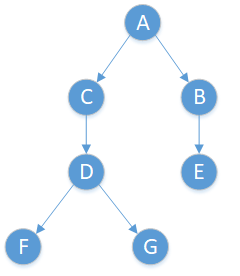
\includegraphics[width=0.3\textwidth]{Figure/1_1.png}
	\caption{Shortest path tree}
	\label{fig:fig2}
\end{figure}
\subsection{Annotate the tree in part(a) with the order vertives are visited in your BFS.}
\noindent \emph{Answer} : The annotated graph is shown as Fig.\ref{fig:fig3}
\begin{figure}[h]
	\centering
	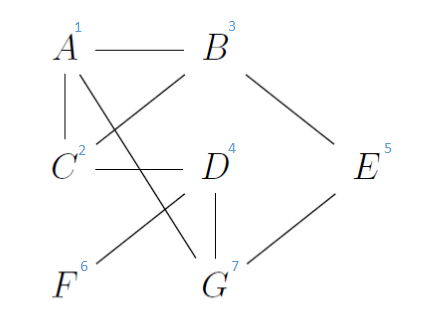
\includegraphics[width=0.3\textwidth]{Figure/1_2.png}
	\caption{Annotated graph}
	\label{fig:fig3}
\end{figure}
\subsection{List the cross-edges of the BFS.}
\noindent \emph{Answer} : The cross edges of the BFS could be described as follows:
\begin{equation*}
	\{(B,C)\}
\end{equation*}


\section{Warm-up: Topological Sorting}
\begin{figure}[h]
	\centering
	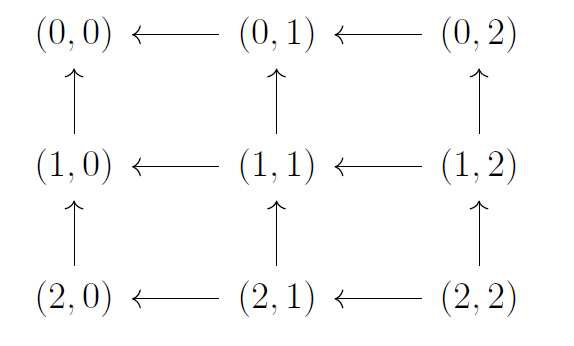
\includegraphics[width=0.4\textwidth]{Figure/2.png}
	\label{fig:fig4}
\end{figure}
\subsection{Find four distinct topological ordering of the nodes in the following directed acyclic graph, presented here as a $3\times3$ grid.}
\noindent\emph{Answer} : The topological ordering of the nodes could be:
\begin{enumerate}
	\item $\{(2,2),(2,1),(1,2),(2,0),(1,1),(0,2),(1,0),(0,1),(0,0)\}$
	\item $\{(2,2),(1,2),(2,1),(2,0),(1,1),(0,2),(1,0),(0,1),(0,0)\}$
	\item $\{(2,2),(2,1),(1,2),(2,0),(0,2),(1,1),(1,0),(0,1),(0,0)\}$
	\item $\{(2,2),(2,1),(2,0),(1,2),(0,2),(1,1),(1,0),(0,1),(0,0)\}$
\end{enumerate}
\subsection{Describe how to generalize your orderings to the case of a graph with the same connectivity pattern on an $n\times n$ grid.}
\noindent\emph{Answer} : As is shown in Fig.\ref{fig:fig5}, the nodes can be classified into $5$ different classes according to their depth from the starting node ${(2,2)}$. As we can see from the graph, the two indexes of the nodes is always larger or equal than $0$, and the deeper the node is, the less the sum of two indexes would be. This observation also corresponds to the classification we made as above. Since the nodes in the same class have the same depth from the starting node, we can arrange them randomly (in class) in the topological order. However, as to the ordering between different classes, we can only follow the order from the starting node to the end point. 
\begin{figure}[h]
	\centering
	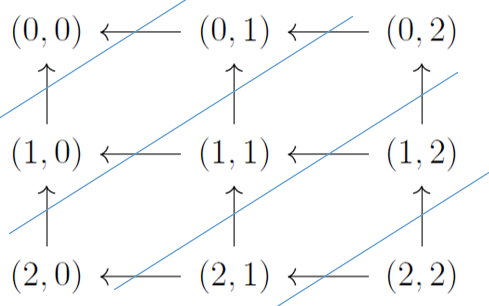
\includegraphics[width=0.4\textwidth]{Figure/2_1.png}
	\caption{Classify the nodes}
	\label{fig:fig5}
\end{figure}

To describe the topological order, we define \textbf{class(n)} as the nodes which have their two indexes' sum is $n$. For example, $class(n) = \{(n,0),(n-1,1),...,(1,n-1),(0,n)\}$. Thus, the topological order for an $n\times n$ grid would be: $\{class(n),class(n-1),...,class(0)\}$. One thing to node here is the $class(n)$ does not necessarily mean a ordered set, so that it could generate $n!$ possible orderings. As to the $n\times n$ grid, the number of possible ordering is $\prod_{i=0}^{n}n!$.

\section{A Unicycle Problem}

Prove that a cycle exists in an undirected graph if and only if a BFS of that graph has a cross-edge. Your proof may use the following facts from graph theory:
\begin{enumerate}
	\item There exists a unique path between any two vertices of a tree.
	\item Adding any edge to a tree creates a unique cycle.
\end{enumerate}

\noindent\emph{Proof} : 

($\Longrightarrow$): Since the BFS of a graph will build a tree according to the nodes' distance from the starting node, the depths of nodes is the same as their distance from the starting node. However, if their is a cross-edge in the BFS search tree, it means there is at least one edge in the graph except the BFS search tree. According to the fact 2 provided by the question, there is a circle in the graph.

($\Longleftarrow$): Since there is a cycle exists in the undirected graph, there is at least two different paths from nodes in the cycle, say $A$ and $B$. However, as the fact 1 provided, the BFS tree will only cover one unique path between $A$ and $B$. And there is also another path from $A$ to $B$ in the graph, which means there is at least one cross-edge with one end is either $A$ or $B$. So that the BFS of that graph has a cross-edge.

Based on the discussion above, the statement made by the question stands.

\section{A Bicycle Problem}
\textbf{C-13.15} : Let $G$ be an undirected graph with $n$ vertices and $m$ edges. Describe an $O(n+m)$ time algorithm to determine whether $G$ contains at least two cycles.
\noindent\emph{Answer} : To solve this problem, we can perform DFS search on the graph and return a number of cycle detected. To determine a cycle, we need to maintain a list of visited vertices to indicate the order of DFS. Once we have reached a vertice that have already been visited, that means we detected a cycle. The algorithm is shown as follows:
\begin{algorithmic}
	\State \textbf{Algorithm} DetectCycle($V,E,n,m$)
	\State \textbf{Input}: $n$ vertices $V$, and $m$ edges $E$. The graph is represented by link list. The link list is named as $link$ with size of $links$
	\State \textbf{Output}: The number of cycles detected.
	\State 
	\State $visited\gets$ empty bool list with length of $n$ and initial value of False
	\State $smallest\gets \infty$
	\For{$i\gets0$ to $n$}
		\If {$indegree(V[i])<smallest$}
			\State $smallest\gets indegree(V[i])$
			\State $start\gets i$ \Comment Let the node with smallest $in$ $degree$ to be the start
		\EndIf
	\EndFor
	\State \Return DFS($start$) \Comment Start from the initial node.
	\State 
	\State \textbf{def} DFS($x$) \Comment $x$ is the index of vertice to be search in this call stack
	\If {$x.links = 0$}
	\State \Return $0$
	\Else
	\State $cycles\gets0$
	\For{$i\gets 0$ to $x.links$}
	\If{$visited[x.link[i]]$}
	\State\Return 1;
	\Else
	\State $visited[x.link[i]]\gets$ True 
	\State $cycles\gets cycles +$DFS($x.link[i]$)
	\EndIf
	\EndFor
	\State \Return $cycles$
	\EndIf
\end{algorithmic}


\section{Maximal Independent Set}
An \emph{independent set} $I$ of an undirected graph $G=(V,E)$ is a subset $I\subseteq V$ such that if $u,v \in I$, then $(u,v)\not \in E$. A \emph{maximal independent set} $M$ is an independent set which cannot have any vertices added to it without losing the independent set property. Describe an efficient algorithm to compute the maximal independent set of such $G$.

\noindent\emph{Answer} : The definition of \emph{maximal independent set} $S$ is equivalent to: for $v\in V$, one of the following is true:
\begin{enumerate}
	\item $v\in S$,
	\item $N(v)\cap S \not = \emptyset$, where $N(v)$ denotes the neighbors of $v$.
\end{enumerate}

Thus, using the following method could find a single maximal independent set:
\begin{enumerate}
	\item Initialize $I$ to an empty set,
	\item While $V$ is not empty:
		\subitem Choose a node $v\in V$;
		\subitem Add $v$ to the set $I$;
		\subitem Remove from $V$ the node $v$ and all its neighbors.
	\item Return $I$.
\end{enumerate}

The algorithm could be described as follows:
\begin{algorithmic}
	\State \textbf{Algorithm} MIS($V,E,n,m$)
	\State \textbf{Input}: $n$ vertices $V$, and $m$ edges $E$. The graph is represented by link list. The link list is named as $link$ with size of $links$
	\State \textbf{Output}: The \emph{Maximal independent set} $S$
	\State $S\gets$ empty set
	\While{$not(V.IsEmpty())$}
		\For{\textbf{each} $v\in V$}
			\State $S.append(v)$
			\For{\textbf{each} $neighbor\in v.link$}
				\State $V.remove(neighbor)$
			\EndFor
			\State $V.remove(v)$
		\EndFor
	\EndWhile
\end{algorithmic}

The runtime of this algorithm is $O(m)$ because in the worst case we need to check all edges.
\section{Application: Procrastinator's Sort}
\noindent\emph{Answer} : Since this problem have limited the importance of questions on an integer scale from $1$ to $10$, we can first put the questions into $10$ buckets and then do Topological Sort. The algorithm can be described as follows:
\begin{algorithmic}
	\State \textbf{Algorithm} TopoSortWithOrder($V,E,n,m$)
	\State \textbf{Input}: $n$ vertices $V$, and $m$ edges $E$. The graph is represented by link list. The link list is named as $link$ with size of $links$
	\State \textbf{Output}: The order $S$ of Socrastes to solve questions.
	
	\State $buckets\gets10$ empty lists
	\For{$i\gets0$ to $n$}
		\State $buckets[V[i].weight].append(V[i])$ \Comment Build the buckets
	\EndFor
	
	\While{$V.size>0$} \Comment Not all the questions are in the list
		\State $Flag \gets False$
		\For{$i\gets 1$ to $10$}\Comment Search from the first bucket to the last
			\For{$j\gets 0$ to $bucket[i].size$}
				\If{$bucket[i,j].indegree=0$}\Comment Can be solved
					\State $S.append(bucket[i,j])$
					\State $V.remove(bucket[i,j])$ \Comment Remove the vertice
					\State $E.remove(bucket[i,j])$ \Comment Remove the edges to this vertice
					\State $Flag\gets True$
					\State \textbf{break}
				\EndIf
			\EndFor
			\If{$Flag$}
				\State \textbf{break}
			\EndIf
		\EndFor
	\EndWhile
	\State \Return $S$
\end{algorithmic}

Since in this problem we use buckets to deal with the weights, it will only add constant time to the topological sorting, so that the time complexity is still $O(m+n)$.
\section{Application: Zombie Apocalypse}
\noindent\emph{Answer} : Since the problem did not give any limitations to the runtime, we can complete this problem by brute force:

\begin{algorithmic}
	\State \textbf{Algorithm} FindMaxTime($M,m,n$)
	\State \textbf{Input}: An matrix $M$ as indicated in the question, with $m,n$ as its size.
	\State \textbf{Output}: The time for all humans to become zombies.
	\State $Time\gets$ an $m\times n$ integer matrix with initial value of $0$
	\State $NumberOfHumans\gets0$
	\For{$i\gets 0$ to $n$}
		\For{$j\gets 0$ to $n$}
			\If{$M(i,j)=H$}\Comment This cell is a human
				\State $NumberOfHumans \gets NumberOfHumans + 1$
			\EndIf
			\If{$M(i,j)=Z$}
				\State $Time(i,j)=0$ \Comment Mark initial zombie as infected in time 0
			\EndIf
		\EndFor
	\EndFor
	\State
	\State $CurrentTime \gets 1$
	\While{$NumberOfHumans>0$}\Comment Start the spread
		\For{$i\gets 0$ to $n$}
			\For{$j\gets 0$ to $n$}
				\If{$M(i,j)=Z$}\Comment This cell is a zombie
					\If{$M(i-1,j)=H$} \Comment Four directions of spread
						\State $NumberOfHumans\gets NumberOfHumans -1$
						\State $Time(i-1,j)=CurrentTime$ 
					\EndIf
					\If{$M(i,j-1)=H$}
						\State $NumberOfHumans\gets NumberOfHumans -1$
						\State $Time(i,j-1)=CurrentTime$ 
					\EndIf
					\If{$M(i+1,j)=H$}
						\State $NumberOfHumans\gets NumberOfHumans -1$
						\State $Time(i+1,j)=CurrentTime$ 
					\EndIf
					\If{$M(i,j+1)=H$}
						\State $NumberOfHumans\gets NumberOfHumans -1$
						\State $Time(i,j+1)=CurrentTime$ 
					\EndIf
				\EndIf
			\EndFor
		\EndFor
		\State $CurrentTime\gets CurrentTime +1$
	\EndWhile
	\State
	\State $MaxTime \gets 0$
	\For{$i\gets 0$ to $n$}
		\For{$j\gets 0$ to $n$}
			\If{$M(i,j)=Z$}
				\If{$Time(i,j)>MaxTime$}
					\State $MaxTime \gets Time(i,j)$
				\EndIf
			\EndIf
		\EndFor
	\EndFor
	\State \Return $MaxTime$
\end{algorithmic}
\section{EECS454 only}
\subsection{R-17.2}
Use a truth table to convert the Boolean formula $B=(a\leftrightarrow(b+c))$ into an equivalent formula in CNF. Show the truth table and the intermediate DNF formula for $\overline{B}$

\noindent\emph{Answer} : The truth table can be shown as follows Table.\ref{tab:tab1}
\begin{table}[!hbp]
	\centering
	\caption{Truth table for $B$}
	\begin{tabular}{c|c|c|c}
		\hline 
		\hline
		a	&b	&c	&$B=(a\leftrightarrow(b+c))$\\
		\hline
		0	&0	&0	&1	\\
		\hline
		0	&0	&1	&0	\\
		\hline
		0	&1	&0	&0	\\
		\hline
		0	&1	&1	&1	\\
		\hline
		1	&0	&0	&0	\\
		\hline
		1	&0	&1	&1	\\
		\hline
		1	&1	&0	&0	\\
		\hline
		1	&1	&1	&1	\\
		\hline
		\hline
		\end{tabular}
		\label{tab:tab1}
\end{table}

So that the CNF formula for $B=(a+b+\overline{c})\cdot(a+\overline{b}+c)\cdot(\overline{a}+b+c)\cdot(\overline{a}+\overline{b}+c)$, and the DNF formula for $\overline{B}=(\overline{a}\cdot\overline{b}\cdot c)+(\overline{a}\cdot b\cdot\overline{c})+(a\cdot\overline{b}\cdot\overline{c})+(a\cdot b\cdot\overline{c})$.

\subsection{C-17.7}
Consider the 2SAT version of the CNF-SAT problem, in which every clause in the given formula $S$ has exactly two literals. Note that any clause of the form $(a + b)$ can be thought of as two implications, $(\overline{a} \rightarrow b)$ and $(\overline{b} \rightarrow a)$. Consider a graph $G$ from $S$, such that each vertex in $G$ is associated with a variable, $x$, in $S$, or its negation, $\overline{x}$. Let there be a directed edge in $G$ from $\overline{a}$ to $b$ for each clause equivalent to $(\overline{a} \rightarrow b)$. Show that $S$ is not satisfiable if and only if there is a variable $x$ such that there is a path in $G$ from $x$ to $\overline{x}$ and a path from $\overline{x}$ to $x$. Derive from this rule a polynomial-time algorithm for solving this special case of the CNF-SAT problem. What is the running time of your algorithm?

\noindent\emph{Answer} : 
	First we need to prove the iff:
	
	($\Longrightarrow$): Since there is a path from $x$ to $\overline{x}$ and an other path from $\overline{x}$ to $x$, it can be simply concluded that $G$ is equivalent to $(\overline{x}\rightarrow x)\cdot(x\rightarrow\overline{x})$, which is the same as $(x+x)=x$. However, it is only related to one literal, which is contradict to the definition of $S$, so that $S$ is not satisfied.
	
	($\Longleftarrow$): Since we know $S$ is not satisfiable, we can conclude that the graph $G$ can be derived into a expression that is only related to $x$, because the nodes in $G$ is related to either $x$ or $\overline{x}$. Thus, we can assert that $G$ can be represented by $(\overline{x}\rightarrow x)\cdot(x\rightarrow\overline{x})$ because the directed edges in $G$ can only be represented in ways like $(a\rightarrow b)$. $(\overline{x}\rightarrow x)\cdot(x\rightarrow\overline{x})$ is equivalent to a path from $x$ to $\overline{x}$ and an other path from $\overline{x}$ to $x$.
	
	The polynomial-time algorithm is described as follows: Suppose the two literals are $a and b $. First, try $a=0,b=0$, then try $a=1,b=0$, then $a=0,b=1$, finally $a=1,b=1$. By enumerating all the possible cases for $a$ and $b$, we can examine whether this 2SAT problem can be satisfied. The running time of this algorithm is $O(1)$.
\subsection{C-17.8}
Suppose an oracle has given you a magic computer, $C$, that when given any Boolean formula $B$ in CNF will tell you in one step whether $B$ is satisfiable. Show how to use $C$ to construct an actual assignment of satisfying Boolean values to the variables in any satisfiable formula $B$. How many calls do you need to make to $C$ in the worst case in order to do this?

\noindent\emph{Answer} : 
	Suppose the Boolean formula $B$ have $n$ different literals, we can then enumerate all possible cases for these $n$ different literals and use $C$ to examine whether they can satisfy $B$. Since there are $2^n$ different cases for $C$ to compute, we need to call $C$ for $2^n$ times.
\end{document}